\begin{savequote}[150mm] 
There are only two hard things in Computer Science: cache invalidation, naming things and off-by-1 errors. \qauthor{Phil Karlton}
\end{savequote}

\chapter{Background \label{chap2:background}}
This chapter provides insights from literature on both outlier detection in Section \ref{sec2:outlier} and web-scale techniques in Section \ref{sec2:webscale}.

\section{Outlier detection algorithms \label{sec2:outlier}}
Outlier detection algorithms aim to automatically identify valuable or disturbing observations in large collections of data. First, we identify the different classes of machine learning algorithms \cite{Fayyad:1996:DMK:257938.257942}, which also applies for outlier detection algorithms:

\paragraph{Unsupervised} algorithms try to find a hidden structure or pattern within a set of unlabeled observations. As illustrated in Figure \ref{fig:unsupervised}, the observations given as the input of the algorithm are unlabeled, so no assumptions can be made. For example, $k$-means clustering, which is a classical example of unsupervised clustering, can be applied on a set of observations to extracts $k$ cluster heads. The set of observations is reduced to a set of cluster heads which can be reviewed or used as input for the next algorithm. In the case of clustering, it is not clear how many clusters are hidden in the observations. This makes it often hard to evaluate performance of unsupervised algorithms as in the case of the example the error function depends of the value of $k$. For each problem and dataset it is important to select the appropriate distance measure as the results are as good as the distance measure can differentiate the observations.

\begin{figure}[ht!]
\centering
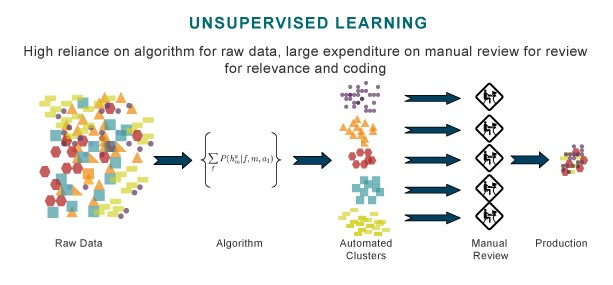
\includegraphics[width=\textwidth]{figures/unsupervised.jpg}
\caption{Unsupervised learning}
\label{fig:unsupervised}
\end{figure}

\paragraph{Supervised} is the machine learning task of inferring a function from labeled training data \cite{9780262018258}. As depicted in Figure \ref{fig:supervised}, supervised methods require as input set observations accompanied by a label which indicates to which class each observation belongs (for example, a label which is either legitimate or fraudulent) in order to assign the observation to a specific class. The training-set is used by the algorithm to learn how to separate the different classes. Based on the input the algorithm will learn a function to distinguish the different classes. Once the model is trained, it can be used to classify to an observation of which the label is not known yet. A disadvantage of supervised learning with respect to outlier detection is that large amount of labeled data is needed to train the model, which is not always available. 

\begin{figure}[ht!]
\centering
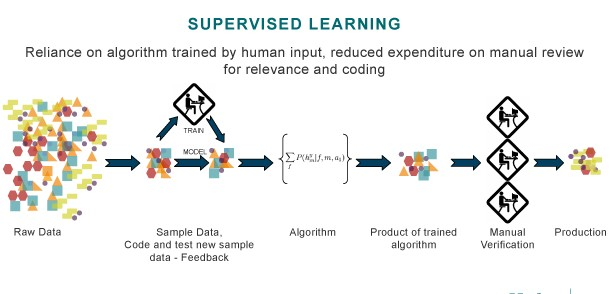
\includegraphics[width=\textwidth]{figures/supervised.jpg}
\caption{Supervised learning}
\label{fig:supervised}
\end{figure}

\paragraph{Semi-supervised} learning is a class between unsupervised and supervised learning. The algorithms consists of a supervised algorithm that makes use of typically a small amount of labeled data with a large amount of unlabeled data. First the model is trained using the labeled data, once done the model is further trained by bootstrapping the unlabeled data. The unlabeled data is presented to the algorithm and subsequently the algorithm is trained based on the prediction of the algorithm.

The next step in the process is to detect outliers based on the stream of observations. The outliers might tell something about the transaction in order to determine whether it is legit or possibly fraudulent. This information can be used when a financial transaction is made. Within a short amount of time it needs to be determined whether the transaction is trustworthy, if not the transaction may be canceled real time.

The goal of outlier detection is to identify the observations that, for some reason, do not fit well within the remainder of the model. A commonly used rule of thumb is that observations deviating more than three times the standard deviation from the distribution are considered outliers \cite{9783540262565}. Obviously this is not a very sophisticated method as it takes a global decision which is not locally aware. Mostly, such a global outlier model leads to a binary decision of whether or not a given observation is an outlier. Local methods typically compute unbound scores of `outlierness'. These scores differ per algorithm in scale, range and meaning \cite{4053049}, but they can be used to discriminate different levels of outliers or to sort them and separate the top $k$-observations.

Within the literature, different classes of outlier detection algorithms exists:
\begin{description}
 \item[Statistical based] assumes that the given dataset has a distribution model which can be approximated using a function \cite{Hadi2009}. Outliers are those observations that satisfy a discordancy test in relation to the hypothesized distribution \cite{barnett1994outliers}. 
 \item[Distance based] unifies the statistical distribution approach \cite{Knorr:1997:UAM:782010.782021} by assuming that an observation is an inlier when the distance of the $k$-nearest observations is smaller than $\delta$ \cite{Knorr98algorithmsfor}. An updated definition which does not require the distance $\delta$, but introduces $n$ which defines whether point $p$ is an outlier if $n-1$ other observations in the dataset have a higher value for $D^{k}$ \cite{Ramaswamy:2000:EAM:335191.335437}. Where $D^{k}(p)$ is the sum of the distances to the nearest $k$ observations with respect to $p$.
 \item[Density based] algorithms identify an observation as an outlier if the neighbourhood of a given observation has a significantly lower density with respect to the density of the neighbouring observations \cite{Breunig:2000:LID:335191.335388,Breunig:2000:LID:342009.335388}.
\end{description}
Besides the above-mentioned classes, there are many domain-specific outlier detection algorithms, for example for tumor detection within MRI data \cite{991693} or algorithms that detect interesting observations within engineering data \cite{rog}.

Density-based approaches are sometimes seen as a variant of the distance-based approach as they share characteristics \cite{Kriegel:2008:AOD:1401890.1401946}. Distance based-algorithms consider an observation an outlier when there are fewer than $k$ other observations within $\delta$ distance  \cite{Knorr:1999:FIK:645925.671529,Knorr:2000:DOA:764212.764218}. Another definition is the top $n$-observations which have the highest average distance to $k$ nearest neighbours \cite{fastoutlier,Eskin02ageometric}. Density-based algorithms take this one step further as they compute from the $k$-nearest observations their average distance to their $k$-nearest observations and compare them with their own distance to the $k$-nearest observations \cite{Schubert:2014:LOD:2560809.2560914}.

With respect to all available algorithm in literature, a subsection is presented in Table \ref{tbl:overviewAlgorithms} based on the restrictions:
\begin{itemize}
  \item The algorithm must be general-purpose and not only applicable within a specific domain.
  \item Many classical statistical algorithms, which are limited to one or only a few dimensions \cite{overviewsurvey}, have been left out as they are not applicable anymore.
  \item The observations that are the input data of the algorithm consist of a $m$-dimensional continues feature vector ${\bf x}=[x_{1},\ldots,x_{m}] \in \mathbb{R}^{m}$.
\end{itemize}

\begin{table}[!ht]
\noindent\makebox[\textwidth]{%
\begin{tabular}{lll}
{\bf Algorithm} & {\bf Type} & {\bf Year} \\ \hline
HilOut \cite{fastoutlier} & Distance-based & 2002 \\
Local Outlier Factor (LOF) \cite{Breunig:2000:LID:335191.335388,Aggarwal:2003:FCE:1315451.1315460} & Density-based & 2000 \\
Fast-MCD \cite{Rousseeuw:1999:FAM:331435.331458} & Statistical-based & 1999 \\
Blocked Adaptive Computationally Efficient Outlier Nominators \cite{Billor2000279} & Statistical-based & 2000 \\
Local Distance-based Outlier Factor (LDOF) \cite{Zhang2009} & Distance-based & 2009 \\
INFLuenced Outlierness (INFLO) \cite{ranking} & Density-based & 2006 \\
No-name \cite{Ramaswamy:2000:EAM:335191.335437} & Distance-based & 2000 \\
No-name \cite{Bay:2003:MDO:956750.956758} & Distance-Based & 2011 \\
Connectivity-Based-Outlier-Factor (COF) \cite{Tang:2002:EEO:646420.693665} & Density-Based & 2002 \\
Local Outlier Probabilities (LoOP) \cite{Kriegel:2009:LLO:1645953.1646195} & Density-based & 2009\\
Local Correlation Integral (LOCI) \cite{citeulike:1156150} & Distance-based & 2003 \\
Angle-Based Outlier Detection (ABOD) \cite{Kriegel:2008:AOD:1401890.1401946} & Angle-based & 2008 \\
Stochastic Outlier Selection (SOS) \cite{MSU:CSE:00:2} & Distance-based & 2012 \\
Simplified Local Outlier Detection (Simplified-LOF) \cite{Schubert:2014:LOD:2560809.2560914} & Density-based & 2014 \\           
\end{tabular}
}
\caption{An overview of outlier detection algorithms which match the above mentioned criteria. \label{tbl:overviewAlgorithms}}
\end{table}

All of the distance based and density based algorithms stated in Table \ref{tbl:overviewAlgorithms} work with Euclidean distance, which is the most popular distance measure for continuous features. For discrete features, the Euclidean distance could be replaced by the Hamming distance. Also, other asymmetrical distance measures can be used.

A disadvantage of statistical-based approaches is that they are parametric since they try to model the data to a given distribution. The majority of the distance-based methods have a computational complexity of $\mathcal{O}(n^{2})$ as the pair-wire distance between all observations is required which effectively yields an $n$ by $n$ distance matrix. This makes it difficult to apply the algorithm to very large datasets as the execution time grows quadratic which is not feasable for large datasets. A way to reduce the computational time is by using spatial indexing structures such as the KD-tree \cite{Bentley:1975:MBS:361002.361007}, R-tree \cite{Guttman:1984:RDI:971697.602266}, X-tree \cite{Berchtold:1996:XIS:645922.673502} or another variation. The problem using such optimized data structures is the difficulty to distribute the data structure across multiple machines.

Unfortunately the `curse of dimensionality' also applies to $\epsilon$-range queries and $k$-nearest neighbour search \cite{citeulike:12369622}. The effect of the dimensionality manifests itself as the number of dimensions increases and the distance to the nearest data point approaches the distance to the farthest observation \cite{Beyer99whenis}. When taking this to an extreme, as in Equation \ref{eq:distlimit}, where $\text{dist}_{\text{max}}$ is the maximum distance to origin, and $\text{dist}_{\text{min}}$ the minimum. When using an infinite number of vector, the distance between the vectors will approach zero \cite{Hinneburg:2000:NNH:645926.671675}. The distance between them becomes less meaningful as the dimensionality increases and the difference between the nearest and the farthest point converges to zero \cite{meaningnearestneighbour,Hinneburg:2000:NNH:645926.671675,Aggarwal01onthe}.

\begin{equation}
\lim_{d \to \infty} \frac{\text{dist}_{\text{max}} - \text{dist}_{\text{min}}}{\text{dist}_{\text{min}}} \to 0
\label{eq:distlimit}
\end{equation}

Higher dimensionality not only hinders in discriminating the distance between the different observations, it also makes the outliers less intuitive to understand. For distance-based outlier algorithms, there are ways to evaluate the validity of the identified outliers which helps to improve the understanding of the data \cite{Knorr:1999:FIK:645925.671529}. As the number of dimensions grows, this process becomes difficult and impossible in extremes.

The use of high-dimensional data depends on the context and cannot be generalized. High-dimensional data can improve accuracy when all the dimensions are relevant and the noise is tolerable.

Another option is to reduce the number of dimensions, which means converting data of high dimensionality into data of much lower dimensionality such that each of the lower dimensions convey much information. Typical techniques that are used are Principal Component Analysis and Factor analysis \cite{citeulike:5467879}. There are more sophisticated techniques which focus on removing the noisy features which do not add any value to the result or even introduce noise \cite{ca37f828023c4aa290d8c6f9f809cab2}, but this is outside the scope of the thesis.

\section{Web-scale computing \label{sec2:webscale}}

In order to allow a system to scale, which is required to cope with the increasing workload, as well as to be able to process large amounts of data which does not fit on a single machine, web-scale technology is adopted. This typically involves the ability to seamlessly provision and add resources to the distributed computing environment. Web-scale is often associated with the infrastructure required to run large distributed applications such as Facebook, Google, Twitter, LinkedIn, etc. 

Within literature, different definitions of cloud-computing have been proposed \cite{clouddef}, there is diversity here, as cloud-computing does not comprise a new technology, but rather a new model that brings together a set of existing technologies in order to develop and execute applications in a way that differs from the traditional approach \cite{zhang:cloud}. Web-scale architecture is an active field of research \cite{cherniack2003scalable}. Web-scale applications rely on cloud computing which is one of the most significant shifts in modern IT for enterprise applications and has become a powerful architecture to perform large-scale and complex computing. Within literature, several definitions of cloud computing exists \cite{sathyavani}. Clouds are used for different purposes and have numerous application areas. We define a cloud as; `a large pool of easily accessible virtualized resources, which can be dynamically reconfigured to adjust to a variable load, allowing for optimum resource utilization' \cite{Vaquero:2008:BCT:1496091.1496100}. 

On top of the cloud-computing environment big-data techniques are used. The world of big-data consists of a wide range of tools and techniques, which address and solve different problems. A mapping of the different components is given in Figure \ref{fig:classification}. Our focus is on the data-processing as our goal is to efficiently distribute the outlier detection algorithm onto a cluster of working nodes.

\begin{figure}[!ht]
\noindent\makebox[\textwidth]{%
    \begin{tikzpicture}[level 1/.style={sibling distance=40mm},edge from parent/.style={->,draw},>=latex]
    
    % root of the the initial tree, level 1
    \node[root] {Big Data Classification}
    % The first level, as children of the initial tree
      child {node[level 2] (c1) {Data Sources}}
      child {node[level 2] (c2) {Content Format}}
      child {node[level 2] (c3) {Data Stores}}
      child {node[level 2] (c4) {Data Staging}}
      child {node[level 2] (c5) {Data Processing}};
    
    \node [style=level 3, below of = c1, xshift=15pt] (c11) {Web and Social};
    \node [style=level 3, below of = c11] (c12) {Machine};
    \node [style=level 3, below of = c12] (c13) {Sensing};
    \node [style=level 3, below of = c13] (c14) {Transaction};
    \node [style=level 3, below of = c14] (c15) {Internet of Things};
    
    \node [style=level 3, below of = c2, xshift=15pt] (c21) {Structured};
    \node [style=level 3, below of = c21] (c22) {Semi-structured};
    \node [style=level 3, below of = c22] (c23) {Unstructured};
    
    \node [style=level 3, below of = c3, xshift=15pt] (c31) {Document-store};
    \node [style=level 3, below of = c31] (c32) {Column-oriented};
    \node [style=level 3, below of = c32] (c33) {Graph-based};
    \node [style=level 3, below of = c33] (c34) {Key-value};
    
    \node [style=level 3, below of = c4, xshift=15pt] (c41) {Cleaning};
    \node [style=level 3, below of = c41] (c42) {Normalization};
    \node [style=level 3, below of = c42] (c43) {Transform}; 
    
    \node [style=level 3, below of = c5, xshift=15pt] (c51) {Batch};
    \node [style=level 3, below of = c51] (c52) {Real-time};
    
    \foreach \value in {1,2,3,4,5}
      \draw[->] (c1.195) |- (c1\value.west);
    
    \foreach \value in {1,2,3}
      \draw[->] (c2.195) |- (c2\value.west);
    
    \foreach \value in {1,2,3,4}
      \draw[->] (c3.195) |- (c3\value.west);
      
    \foreach \value in {1,2,3}
      \draw[->] (c4.195) |- (c4\value.west);
      
    \foreach \value in {1,2}
      \draw[->] (c5.195) |- (c5\value.west);
    \end{tikzpicture}}
      
    \caption{Overview Big-Data landscape \cite{Hashem201598} \label{fig:classification}}
\end{figure}

It started in 2008 when Google introduced the MapReduce computing model which provides a model for processing large datasets in a parallel and distributed fashion on a cluster of machines \cite{Dean:2008:MSD:1327452.1327492}. Google used it to scale their PageRank algorithm to serve personalized results to the users of their search engine \cite{Bahmani:2011:FPP:1989323.1989425}. The MapReduce model is a simple yet powerful model for parallelizing data processing. 

Subsequently in 2007 Microsoft launched a data-processing system to write efficient parallel and distributed applications more easily under the codename Dryad \cite{export:63785}. DryadLINQ provides a set of language extensions that enable a new programming model for large scale distributed computing. A DryadLINQ program is a sequential program composed of LINQ expressions performing arbitrary side-effect-free transformations on datasets \cite{export:70861}. In November 2011 active development on Dryad had been discontinued, and Microsoft shifted their focus to the Apache Hadoop project \cite{linqdisc}.

The Apache Hadoop project is an implementation of the MapReduce model. It is the open-source implementation primarily developed by Yahoo, where it runs jobs that produce hundreds of terabytes of data on at least 10,000 cores \cite{HadoopMapYahoo}. Since then it has been adopted by a large variety of institutes and companies in educational or production uses, among which Facebook, Last.FM and IBM\footnote{Hadoop: PoweredBy \url{https://wiki.apache.org/hadoop/PoweredBy}}.

Although the name MapReduce originally referred to the proprietary Google technology, over the years it became the general term for the way of doing large scale computations. The open-source implementation that has support for distributed shuffles is part of Apache Hadoop\footnote{Apache Hadoop \url{http://hadoop.apache.org/}}. A MapReduce job consists of three phases, namely Map, Combiner and Reduce \cite{Dean:2008:MSD:1327452.1327492}:

\begin{description}
  \item[Map] In the map phase operations on every individual record in the dataset can be performed. This phase is commonly used to transform fields, apply filters or join and grouping operations. There is no requirement that for every input record there should be one output record.
  \item[Combine] For efficiency and optimization purposes it sometimes makes sense to supply a combiner class to perform a reduce-type function. If a combiner is used then the map key-value pairs are not immediately written to the output. Instead they are collected in lists, one list per each key value. When a certain number of key-value pairs have been written, this buffer is flushed by passing all the values of each key to the combiner method and outputting the key-value pairs of the combine operation as if they were created by the original map operation.
  \item[Reduce] Before the reduce task it might be the case that distributed data needs to be copied to the local machine. When this is done, each key with its corresponding values is passed to the reduce operation. 
\end{description}

First, input data is divided into parts and then passed to the mapper which executes in parallel. The result is partitioned by key and locally sorted. Results of the mapper-data with the same key are send to the same reducer and consolidated there. The merge sort happens at the reducer, so all keys arriving at the same reducer are sorted. 

There is a variety of open-source frameworks based or inspired on the MapReduce model, each with their own characteristics, which are commonly used for big-data processing:
\begin{description}
    \item[Apache Hadoop] is the open-source implementation of the propriety MapReduce model. The Apache Hadoop consists of four modules: first, the Hadoop MapReduce framework, which consists of a YARN-based system for the parallel processing of large datasets. Second, the Hadoop Distributed File System (HDFS) in a distributed user-level file system which focuses on portability across heterogeneous hardware and software platforms \cite{5452045} inspired by the Google File System \cite{Ghemawat:2003:GFS:1165389.945450}. Third, Hadoop YARN, which stands for Yet Another Resource Negotiator and is a framework for job scheduling and cluster resource management \cite{Vavilapalli:2013:AHY:2523616.2523633} and, last, Hadoop Common which provides the services for supporting the Hadoop modules.
    \item[Apache Spark] is the implementation of the concept of the Resilient Distributed Datasets (RDDs) developed at UC Berkeley \cite{180560}. RDDs are fault-tolerant, parallel data structures that persist intermediate results in memory and enable the developer to explicitly control the partitioning in order to optimize data locality. Manipulating RDDs can be done using filters, actions and transformations by a rich set of primitives. The concept of RDD is inspired by MapReduce and Dryad.
\end{description}

MapReduce is deficient in iterative jobs because the data is loaded from disk on each iteration and interactive analysis, and significant latency occurs because all the data has to be read from the distributed file system \cite{Zaharia:2010:SCC:1863103.1863113}. This is where Apache Spark steps in by storing intermediate results in-memory.

Hadoop provides fault-tolerance by using the underlying HDFS which replicates the data over different nodes. Spark does not store the transformed information between each step, but when a block of data gets lost, the original data is loaded and Spark reapplies all the transformations, although it is possible to explicit save the state by enforcing a checkpoint. By the use of this strategy Spark's in-memory primitives provide performance up to 100 times faster than Hadoop for certain applications \cite{Xin:2013:SSR:2463676.2465288}.